\documentclass[11pt,a4paper]{article}

\usepackage[utf8]{inputenc}
\usepackage[T1]{fontenc}
\usepackage{mathpazo}
\usepackage[scaled=0.92]{helvet}
\usepackage[margin=1in]{geometry}
\usepackage{graphicx}
\usepackage{amsmath,amssymb,amsfonts}
\usepackage{booktabs}
\usepackage{tabularx}
\usepackage{setspace}
\usepackage{titlesec}
\usepackage{fancyhdr}
\usepackage{float}
\usepackage{caption}

\usepackage{tikz}
\usetikzlibrary{shapes.geometric, arrows.meta, positioning, calc, shadows, backgrounds}
\usepackage[hidelinks]{hyperref}

\setstretch{1.15}
\setlength{\parindent}{0pt}
\setlength{\parskip}{8pt}
\sloppy

\titleformat{\section}{\normalfont\large\bfseries\sffamily}{\thesection}{1em}{}
\titleformat{\subsection}{\normalfont\normalsize\bfseries\sffamily}{\thesubsection}{1em}{}

\pagestyle{fancy}
\fancyhf{}
\fancyhead[L]{\small\sffamily Pengantar Konsep Basis Data Relasional}
\fancyhead[R]{\small\sffamily\thepage}
\renewcommand{\headrulewidth}{0.4pt}

\captionsetup{font=small,labelfont=bf,labelsep=period}

\renewenvironment{abstract}
{\small
	\begin{center}\textbf{\sffamily Abstract}\end{center}
	\begin{quote}}
	{\end{quote}}

\title{\vspace{-1.5cm}\textbf{\sffamily\LARGE Pengantar Konsep Basis Data Relasional:\\ Dari Data Mentah Menuju Sistem Terstruktur}}
\author{
	\textbf{Muhammad Riduwan Khafidi} \\
	\small Program Studi Teknik Rekayasa Perangkat Lunak \\
	\small Politeknik Negeri Batam \\
	\small \texttt{4342611034@students.polibatam.ac.id}
}
\date{\small\today}

\begin{document}

\maketitle
\thispagestyle{empty}

\begin{abstract}
	Basis data (database) merupakan teknologi fundamental yang menopang hampir seluruh sistem digital di era modern. Mulai dari aplikasi e-commerce, sistem pemetaan, portal akademik, hingga analisis performa klub sepak bola, semuanya bergantung pada pengelolaan data yang efisien. Makalah ini membedah konsep dasar basis data sebagaimana dipaparkan dalam modul pengantar basis data. Pembahasan dimulai dari perbedaan mendasar antara \textit{datum} dan \textit{data}, definisi basis data, tujuan perancangannya, keterbatasan penyimpanan konvensional (seperti Excel), hingga konsep Basis Data Relasional (RDB) beserta tahapan perancangannya. Melalui visualisasi diagram yang komprehensif, makalah ini bertujuan untuk memberikan pemahaman holistik mengenai bagaimana data mentah diubah menjadi informasi yang terstruktur dan bernilai guna.
\end{abstract}

\section{Pendahuluan: Basis Data Ada di Mana-Mana}

Pernahkah kita menyadari bahwa setiap aplikasi yang kita gunakan saat ini—mulai dari \textit{e-commerce} seperti Shopee, aplikasi peta seperti Google Maps, sistem informasi akademik kampus, hingga media sosial—tidak bisa berjalan tanpa adanya basis data? Basis data bersifat \textit{ubiquitous} (ada di mana-mana). Perusahaan raksasa seperti Google dan Facebook membangun pusat data (\textit{data center}) raksasa yang berisi ribuan server untuk menyimpan miliaran baris data pengguna mereka.

Penggunaan data tidak hanya terbatas pada aplikasi digital. Dalam dunia olahraga, klub sepak bola Liverpool FC menggunakan analisis \textit{data science} yang luar biasa untuk membantu pelatih mengambil keputusan taktis di tengah pertandingan secara \textit{real-time}. Hal ini menegaskan satu hal: data adalah "minyak baru" (\textit{data is the new oil}) yang harus ditambang, diolah, dan didistribusikan agar memiliki nilai.

\section{Datum vs Data: Memahami Atom Informasi}

Sebelum melangkah lebih jauh, kita harus memahami perbedaan antara \textit{datum} dan \textit{data}. Secara etimologis, kata "data" merupakan bentuk jamak dari kata Latin "datum". Sebuah \textit{datum} adalah satu fakta tunggal, satu entitas, atau satu titik materi yang direkam. Sementara itu, data adalah kumpulan dari fakta-fakta yang direkam tersebut. Data pada dasarnya tidak memiliki arti sebelum diinterpretasikan.

Sebagai ilustrasi, perhatikanlah alur transformasi pada Gambar \ref{fig:datum} di bawah ini. Angka "100" atau kata "Baik" hanyalah sebuah \textit{datum} jika berdiri sendiri. Namun, ketika kumpulan \textit{datum} tersebut dikaitkan dengan konteks kolom (misalnya, Sekolah A memiliki 100 siswa dengan kondisi Baik), barulah ia berevolusi menjadi sebuah informasi yang bermakna.

\begin{figure}[H]
	\centering
	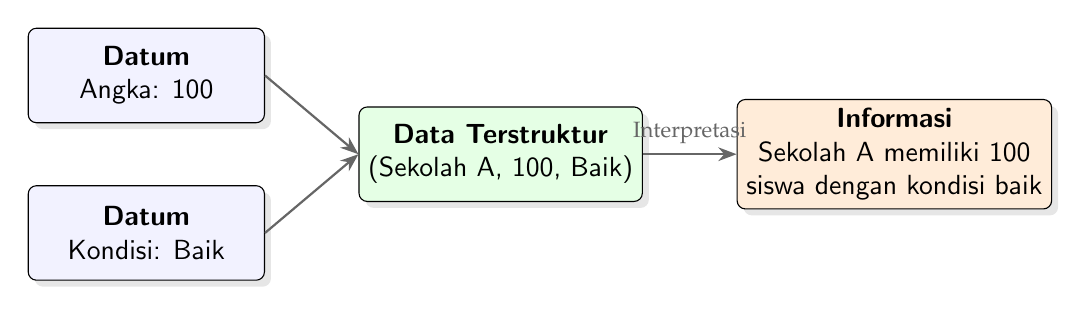
\begin{tikzpicture}[
			node distance=2cm,
			box/.style={draw, rectangle, rounded corners=3pt, minimum width=3cm, minimum height=1.2cm, align=center, fill=blue!5, drop shadow={opacity=0.2}, font=\sffamily},
			arrow/.style={->, >=Stealth, thick, color=gray!80!black}
		]
		\node[box] (d1) at (0,2) {\textbf{Datum}\\ Angka: 100};
		\node[box] (d2) at (0,0) {\textbf{Datum}\\ Kondisi: Baik};

		\node[box, fill=green!10] (data) at (4.5,1) {\textbf{Data Terstruktur}\\ (Sekolah A, 100, Baik)};
		\node[box, fill=orange!15] (info) at (9.5,1) {\textbf{Informasi}\\ Sekolah A memiliki 100\\ siswa dengan kondisi baik};

		\draw[arrow] (d1.east) -- (data.west);
		\draw[arrow] (d2.east) -- (data.west);
		\draw[arrow] (data.east) -- (info.west) node[midway, above, font=\footnotesize] {Interpretasi};
	\end{tikzpicture}
	\caption{Ilustrasi Transformasi \textit{Datum} Menjadi Informasi yang Bermakna.}
	\label{fig:datum}
\end{figure}

\section{Definisi dan Tujuan Basis Data}

Secara harfiah, basis data (\textit{database}) adalah gabungan dari kata "data" dan "base" (basis). Basis data didefinisikan sebagai kumpulan data dalam jumlah besar yang diorganisasikan untuk pencarian dan pengambilan kembali secara cepat oleh komputer. Basis data juga memodelkan objek dunia nyata, yang terdiri dari entitas (misalnya: orang atau barang) dan relasi (misalnya: Tony tinggal di Jalan Ahmad Yani).

Mengapa kita membutuhkan basis data? Sistem penyimpanan data memiliki beberapa tujuan utama. Pertama, kecepatan dan efisiensi ruang penyimpanan. Kedua, akurasi data yang dijaga menggunakan batasan data (\textit{data constraints}) agar tidak ada data ganda. Ketiga, ketersediaan (\textit{availability}) dan kelengkapan, di mana jika data belum lengkap, struktur dapat ditambahkan. Keempat, keamanan (\textit{security}) melalui manajemen pengguna. Terakhir, kemampuan untuk dibagikan (\textit{sharability}), memungkinkan banyak pengguna mengakses dan berbagi basis data yang sama secara bersamaan.

\section{Keterbatasan Excel dan Hadirnya Basis Data Relasional}

Sebagai mahasiswa, kita sering menggunakan Microsoft Excel atau Google Sheets untuk menyimpan data. Excel memang simpel, mudah dibagikan, dan mudah untuk melakukan operasi tambah, edit, serta hapus data. Namun, ketika data sudah mencapai ribuan baris (misalnya data mahasiswa Polibatam), Excel mulai menunjukkan kelemahannya. Ukuran file yang membengkak membuat proses pengolahan menjadi lambat, terjadi duplikasi data (\textit{redundancy}), dan yang paling krusial adalah sulitnya menghubungkan data satu dengan yang lain. Misalnya, jika ingin mencari tahu "Siapa saja mahasiswa yang mengambil mata kuliah Basis Data?", kita harus melakukan pencarian manual yang melelahkan. Belum lagi masalah versi data (jika satu orang mengubah data, orang lain mungkin belum melihat perubahannya) dan masalah keamanan (siapa saja bisa mengedit).

Untuk mengatasi masalah ini, muncullah konsep Basis Data Relasional (RDB). RDB mengorganisir data ke dalam tabel-tabel, baris (\textit{records}), dan kolom. Keunggulan utamanya adalah kemampuannya membangun relasi yang terdefinisi dengan baik antar tabel. Tabel-tabel tersebut saling berkomunikasi dan berbagi informasi, sehingga memudahkan pencarian data yang kompleks. RDB menggunakan Structured Query Language (SQL) sebagai bahasa standarnya.

Sebagai ilustrasi relasi, perhatikan Gambar \ref{fig:rdb_tables} di bawah ini. Terdapat tiga tabel terpisah: Tabel Mahasiswa (MHS), Tabel Mata Kuliah (MKUL), dan Tabel Nilai (NILAI). Tabel Nilai bertindak sebagai jembatan yang menghubungkan mahasiswa dengan mata kuliah yang mereka ambil.

\begin{figure}[H]
	\centering
	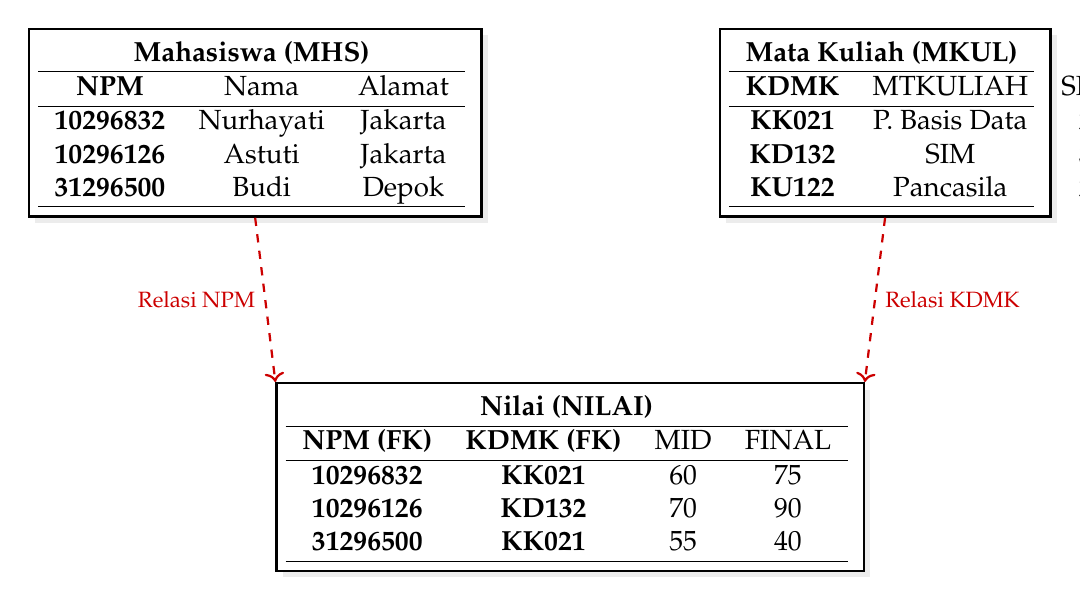
\begin{tikzpicture}[
			table/.style={draw, rectangle, fill=white, thick, align=center, drop shadow={opacity=0.15}},
			header/.style={fill=blue!15, font=\bfseries\sffamily},
			cell/.style={minimum width=1.8cm, minimum height=0.5cm, font=\small\sffamily}
		]
		\node[table] (mhs) at (0,0) {
			\begin{tabular}{c c c}
				\multicolumn{3}{c}{\textbf{Mahasiswa (MHS)}} \\
				\hline
				\textbf{NPM}      & Nama      & Alamat       \\
				\hline
				\textbf{10296832} & Nurhayati & Jakarta      \\
				\textbf{10296126} & Astuti    & Jakarta      \\
				\textbf{31296500} & Budi      & Depok        \\
				\hline
			\end{tabular}
		};

		\node[table] (mkul) at (8,0) {
			\begin{tabular}{c c c c}
				\multicolumn{4}{c}{\textbf{Mata Kuliah (MKUL)}} \\
				\hline
				\textbf{KDMK}  & MTKULIAH      & SKS            \\
				\hline
				\textbf{KK021} & P. Basis Data & 2              \\
				\textbf{KD132} & SIM           & 3              \\
				\textbf{KU122} & Pancasila     & 2              \\
				\hline
			\end{tabular}
		};

		\node[table] (nilai) at (4,-4.5) {
			\begin{tabular}{c c c c}
				\multicolumn{4}{c}{\textbf{Nilai (NILAI)}}           \\
				\hline
				\textbf{NPM (FK)} & \textbf{KDMK (FK)} & MID & FINAL \\
				\hline
				\textbf{10296832} & \textbf{KK021}     & 60  & 75    \\
				\textbf{10296126} & \textbf{KD132}     & 70  & 90    \\
				\textbf{31296500} & \textbf{KK021}     & 55  & 40    \\
				\hline
			\end{tabular}
		};

		\draw[->, dashed, thick, red!80!black] (mhs.south) -- (nilai.north west) node[midway, left, text=red!80!black, font=\footnotesize] {Relasi NPM};
		\draw[->, dashed, thick, red!80!black] (mkul.south) -- (nilai.north east) node[midway, right, text=red!80!black, font=\footnotesize] {Relasi KDMK};
	\end{tikzpicture}
	\caption{Contoh Relasi Antar Tabel dalam Basis Data Relasional.}
	\label{fig:rdb_tables}
\end{figure}

\section{Tahapan Perancangan Basis Data}

Membangun basis data tidak bisa dilakukan secara sembarangan. Terdapat alur perancangan yang sistematis sebelum data dimasukkan ke dalam sistem manajemen basis data (DBMS). Alur ini dimulai dari kebutuhan pengguna hingga menjadi sistem yang siap pakai.

\begin{figure}[H]
	\centering
	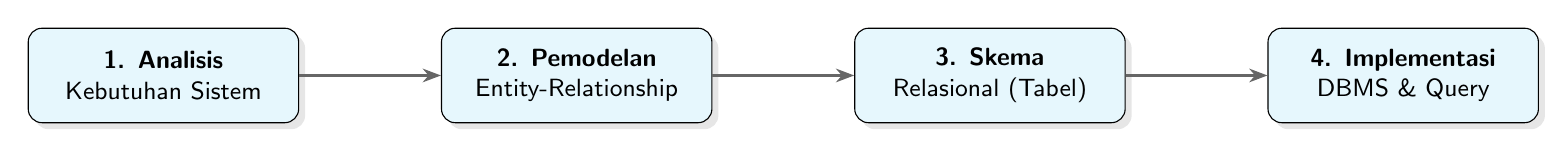
\begin{tikzpicture}[
			node distance=1.8cm,
			block/.style={draw, rectangle, rounded corners=5pt, text width=3.2cm, align=center, minimum height=1.2cm, fill=cyan!10, drop shadow={opacity=0.2}, font=\sffamily\small},
			arrow/.style={->, >=Stealth, thick, color=gray!80!black}
		]
		\node[block] (analisis) {\textbf{1. Analisis}\\ Kebutuhan Sistem};
		\node[block, right=of analisis] (er) {\textbf{2. Pemodelan}\\ Entity-Relationship};
		\node[block, right=of er] (relasi) {\textbf{3. Skema}\\ Relasional (Tabel)};
		\node[block, right=of relasi] (dbms) {\textbf{4. Implementasi}\\ DBMS \& Query};

		\draw[arrow] (analisis) -- (er);
		\draw[arrow] (er) -- (relasi);
		\draw[arrow] (relasi) -- (dbms);
	\end{tikzpicture}
	\caption{Alur Perancangan Basis Data.}
	\label{fig:design_flow}
\end{figure}

Berdasarkan diagram di atas, tahap pertama adalah Analisis Kebutuhan, di mana perancang memahami data apa saja yang perlu disimpan. Tahap kedua adalah membuat Pemodelan Data, biasanya menggunakan Entity-Relationship (ER) Diagram untuk memetakan entitas dan relasinya. Tahap ketiga adalah menerjemahkan model tersebut menjadi Skema Relasional (tabel-tabel). Tahap terakhir adalah implementasi menggunakan perangkat lunak DBMS (seperti MySQL, PostgreSQL, Oracle) dan menuliskan \textit{query} SQL untuk mengelola datanya.

\section{Komponen Ekosistem Basis Data}

Sebuah sistem basis data tidak berdiri sendiri. Ia terdiri dari beberapa komponen yang saling terkait untuk membentuk Sistem Basis Data (\textit{Database System}). Secara garis besar, komponen tersebut meliputi perangkat keras, sistem operasi, basis data itu sendiri, perangkat lunak DBMS (\textit{Database Management System}), pengguna, dan aplikasi pendukung. DBMS bertindak sebagai perantara cerdas yang mengelola data masuk, mengaturnya, dan menyediakan cara agar data tersebut dapat dimodifikasi atau diekstraksi oleh pengguna.

\begin{figure}[H]
	\centering
	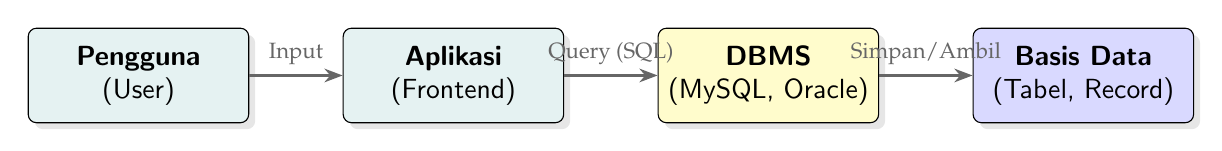
\begin{tikzpicture}[
			box/.style={draw, rectangle, rounded corners=3pt, minimum width=2.8cm, minimum height=1.2cm, align=center, fill=teal!10, drop shadow={opacity=0.2}, font=\sffamily},
			arrow/.style={->, >=Stealth, thick, color=gray!80!black}
		]
		\node[box] (user) at (0,0) {\textbf{Pengguna}\\ (User)};
		\node[box] (app) at (4,0) {\textbf{Aplikasi}\\ (Frontend)};
		\node[box, fill=yellow!20] (dbms) at (8,0) {\textbf{DBMS}\\ (MySQL, Oracle)};
		\node[box, fill=blue!15] (db) at (12,0) {\textbf{Basis Data}\\ (Tabel, Record)};

		\draw[arrow] (user) -- (app) node[midway, above, font=\footnotesize] {Input};
		\draw[arrow] (app) -- (dbms) node[midway, above, font=\footnotesize] {Query (SQL)};
		\draw[arrow] (dbms) -- (db) node[midway, above, font=\footnotesize] {Simpan/Ambil};
	\end{tikzpicture}
	\caption{Interaksi Pengguna, Aplikasi, DBMS, dan Basis Data.}
	\label{fig:dbms_flow}
\end{figure}

\section{Kesimpulan dan Prospek ke Depan}

Memahami konsep dasar basis data adalah fondasi mutlak bagi siapa pun yang ingin terjun ke dunia rekayasa perangkat lunak. Kita telah belajar bahwa data adalah aset berharga yang harus diolah. Dari penyimpanan konvensional yang rentan terhadap redundansi (seperti Excel), kita beralih ke sistem yang lebih tangguh, yaitu Basis Data Relasional, yang mengedepankan hubungan antar entitas melalui tabel-tabel yang terstruktur.

Bidang basis data menawarkan kontribusi besar bagi ilmu komputer dan memiliki prospek karier yang sangat cemerlang. Teknologi ini menjadi pintu gerbang menuju bidang-bidang lanjutan seperti Data Mining, Big Data, Business Intelligence, hingga profesi bergengsi sebagai Data Scientist. Sebagaimana dikatakan oleh David Buckingham, "Data is the new oil. We need to find it, extract it, refine it, distribute it and monetize it." (Data adalah minyak baru. Kita perlu menemukannya, mengekstraknya, memurnikannya, mendistribusikannya, dan memonetisasinya). Basis data adalah kilang minyak tempat kita memurnikan data mentah menjadi informasi yang berharga.

\newpage
\section*{Referensi}
\addcontentsline{toc}{section}{Referensi}

\begin{thebibliography}{99}
	\bibitem{lubis}
	Lubis, A. I. (2026). \textit{Introduction to Database Concepts} [Slide Presentasi Mata Kuliah Pengantar Basis Data]. Politeknik Negeri Batam.

	\bibitem{silberschatz}
	Silberschatz, A., Korth, H. F., \& Sudarshan, S. (2019). \textit{Database System Concepts} (7th ed.). McGraw-Hill Education.

	\bibitem{widyastuti}
	Widyastuti, H. \textit{Slide Relational Database}. [Modul Perkuliahan].

	\bibitem{santiputri}
	Santiputri, M. \textit{Slide Basis Data}. [Modul Perkuliahan].
\end{thebibliography}

\end{document}
